\documentclass[25pt,margin=20mm,innermargin=-6in,blockverticalspace=1mm]{tikzposter}
\geometry{paperwidth=47in,paperheight=33in}
\usepackage[utf8]{inputenc}
\usepackage{amsmath}
\usepackage{amsfonts}
\usepackage{amsthm}
\usepackage{amssymb}
\usepackage{mathrsfs}
\usepackage{graphicx}
\usepackage{caption}
\usepackage{subcaption}
\usepackage{adjustbox}
\usepackage{enumitem}
\usepackage{wrapfig}
\usepackage[backend=bibtex,style=numeric,doi=false,url=false,eprint=false,sorting=none,autocite=superscript]{biblatex}
\usepackage{uofa-theme}
\usetikzlibrary{positioning,shapes,arrows}


\addbibresource{ref.bib}
\AtBeginBibliography{\footnotesize}

% set theme parameters
\tikzposterlatexaffectionproofoff
\usetheme{UofATheme}
\usecolorstyle{UofAStyle}

\title{GRAVI: Gene Regulatory Analysis Using Variable Inputs}
\author{\centering \textbf{Stevie Pederson}\textsuperscript{1,2}, Geraldine Laven-Law\textsuperscript{1}, Richard Iggo\textsuperscript{1,3}, Amy Dwyer\textsuperscript{1}, Theresa E Hickey\textsuperscript{1} and Wayne D Tilley\textsuperscript{1}}
\institute{
  \textsuperscript{1}Dame Roma Mitchell Cancer Research Laboratories, Adelaide Medical School, University of Adelaide\\
  \textsuperscript{2}Black Ochre Data Labs, Telethon Kids Institute\hspace{5mm}
  \textsuperscript{3}Bordeaux Institute of Oncology, University of Bordeaux
}


% begin document
\begin{document}
\maketitle

\node [below right=20mm and 10mm] at (bottomleft |- topright) {
\includegraphics[width=0.08\textwidth]{UoAlogo.png}};
\node [below left=20mm and 10mm] at (topright) {
\includegraphics[width=0.08\textwidth]{tki.jpg}};



\centering

\block{GRAVI Outline}{

	\begin{minipage}{0.08\linewidth}
		
\includegraphics[width=0.8\linewidth]{extraChIPs_sticker}	
	\end{minipage}
	\begin{minipage}{0.82\linewidth}	
	\LARGE
	\centering
	\textbf{GRAVI} is a \texttt{snakemake}\autocite{Molder2021-mo} workflow for performing high-throughput, high-quality Differential Signal Analysis for ChIP-Seq data, exploiting the \texttt{extraChIPs} Bioconductor package.
	GRAVI standardises multiple steps to perform a \textit{complete standalone analysis}, and also enables easier \textit{integration across multiple complex datasets}.
	The workflow can be applied to \textit{one or more} ChIP targets under \textit{two or more} conditions.
	Optional RNA-Seq and HiC data further extend GRAVI to \textbf{directly map dynamic changes in ChIP signal to regulatory targets}.	
	\end{minipage}
	\begin{minipage}{0.09\linewidth}
		\innerblock{\large Find GRAVI on GitHub}{
			\centering
	       	
\includegraphics[width=0.6\linewidth]{gravi-qr-code}		
		}
	\end{minipage}
}

\begin{columns}
    \column{0.33}
    	\block{Key Aims}{
			\Large
		    \begin{enumerate}
		    \item Best Practice Differential ChIP Signal Analysis
		    \item Accurate Mapping of Binding Sites to Regulatory Targets
		    \item Integration of multiple ChIP targets \& treatments
		    \item Highly flexible input data
		    \end{enumerate}    		

    	}
    	\vspace{-1cm}
    	\block{Input Data}{
    		\vspace{-1cm}
    	    \large
    		\begin{minipage}{0.42\linewidth}
    		\innerblock{Minimal Input}{
	    		\begin{itemize}
	    		\item $1\times$ChIP Target (.bam)
	    		\begin{itemize}
	    			\item $2\times$ Conditions	    		
	    		\end{itemize}
	    		\item Gene Annotations (.gtf) 
	    		\item Blacklisted Regions (.bed)
	    		\end{itemize}
	    		
	    	}    	
	    	\vspace{15mm}	
    		\end{minipage}
    		\begin{minipage}{0.58\linewidth}
    		\innerblock{Optional Input}{
    			\begin{itemize}
    			\item Additional ChIP targets/treatments
    			\item Differential Gene Expression (.tsv)
    			\item HiC Interactions (.bedpe)
    			\item Features of Interest (.gtf)
    			\item External Coverage Tracks (.bw)
    			\end{itemize}   		
    			}
    		\end{minipage}
    		\vspace{-1cm}
    	}
    	\block{GRAVI Steps}{
		\large
		\useinnerblockstyle{Table}
		\vspace{-2.5cm}
    		\innerblock[titlewidthscale=0.4,bodywidthscale=0.6]{Always Performed}{
	    		\begin{enumerate}
	    			\item Annotation Preparation
				\item Peak Calling and Sample QC
				\item Differential Signal Analysis
	    		\end{enumerate}
	    	}
	    \vspace{-2cm}
    		\innerblock[titlewidthscale=0.4,bodywidthscale=0.6]{$>$1 Comparison Only}{
			4. Pairwise Comparisons
    		}
    		\vspace{-1cm}

    		
    	}

    	\block{Key Outputs}{
    		\Large
%    		\vspace{-5mm}
%    		A \textit{comprehensive library of results} 
    		
    		\begin{itemize}
    			\item Compiled Multi-Page HTML (Figures, Tables, \texttt{R} Code, etc)
    			\item Bed Files (Peaks, Key Results)
    			\item BigWig Files (Visualisation)
    			\item Spreadsheets (Integrated results with mappings)
    			\item \texttt{R} Data Objects for Custom Downstream Analysis
    		\end{itemize}
    	}


    \column{0.34}
    \useblockstyle{KeyBlockStyle}
    \block{Motivation}{
    \Large
    \vspace{2mm}
    Activation of the Androgen Receptor (AR) induces an \textit{anti-proliferative phenotype} in many breast cancer models\autocite{Hickey2021}.
    Integrating the dynamics of AR binding with the Estrogen Receptor (ER$\alpha$), additional transcription factors, H3K27ac marks and changes in transcription, we were able to investigate the underlying molecular mechanisms.
    Comparison across multiple cancer models was then used to identify key targets and mechanisms.
    \vspace{3mm}
    }
    \useblockstyle{UofABlockStyle}

    \block{Differential Signal Analysis}{
    \useinnerblockstyle{Default}
	\begin{minipage}{0.5\linewidth}
		\innerblock[titlecenter]{Always Performed}{
		    \begin{enumerate}
			    	\item Sliding Windows\autocite{csaw} using either
			    	\begin{enumerate}
			    		\item Quasi-Likelihood Models\autocite{Lund2012-xo}, or
			    		\item SQN\autocite{sqn} with limma-trend\autocite{voom}
			    	\end{enumerate}
			    	\item Range-Based $H_0$\autocite{treat}
			    	\item Independent Hypothesis Weighting\autocite{Ignatiadis2016-cq}
			    	\item Mapped to Genes, Regulatory \mbox{Regions} and Optional Features
			    	\item Tables, Figures and Bed files			    	
			    	\item Enrichment Analysis
%			    	\begin{itemize}
%			    		\item Tables and Network Plots
%			    	\end{itemize}
		    \end{enumerate}
		   }
		\vspace{5mm}
		\innerblock[titlecenter]{If DGE Results Included}{
	    		\begin{enumerate}
			    	\item Direct Targets Identified
			    	\item \textit{Combined} Enrichment Analysis
		    \end{enumerate}
		   }
		\vspace{5mm}
		\innerblock[titlecenter]{Coming Soon}{
		    \begin{enumerate}
			    	\item Fixed-Width Windows
			    	\item More Normalisation Options
			    	\item ATAC-Seq Methods
		    \end{enumerate}
		   }
	\end{minipage}	    
	\begin{minipage}{0.5\linewidth}
		\small
		\centering
    		\begin{tikzfigure}[AR logCPM values A) before and B) after Smooth Quantile Normalisation. AR is translocated from the cytoplasm to the nucleus when activated by DHT\label{fig:logCPM}]
        	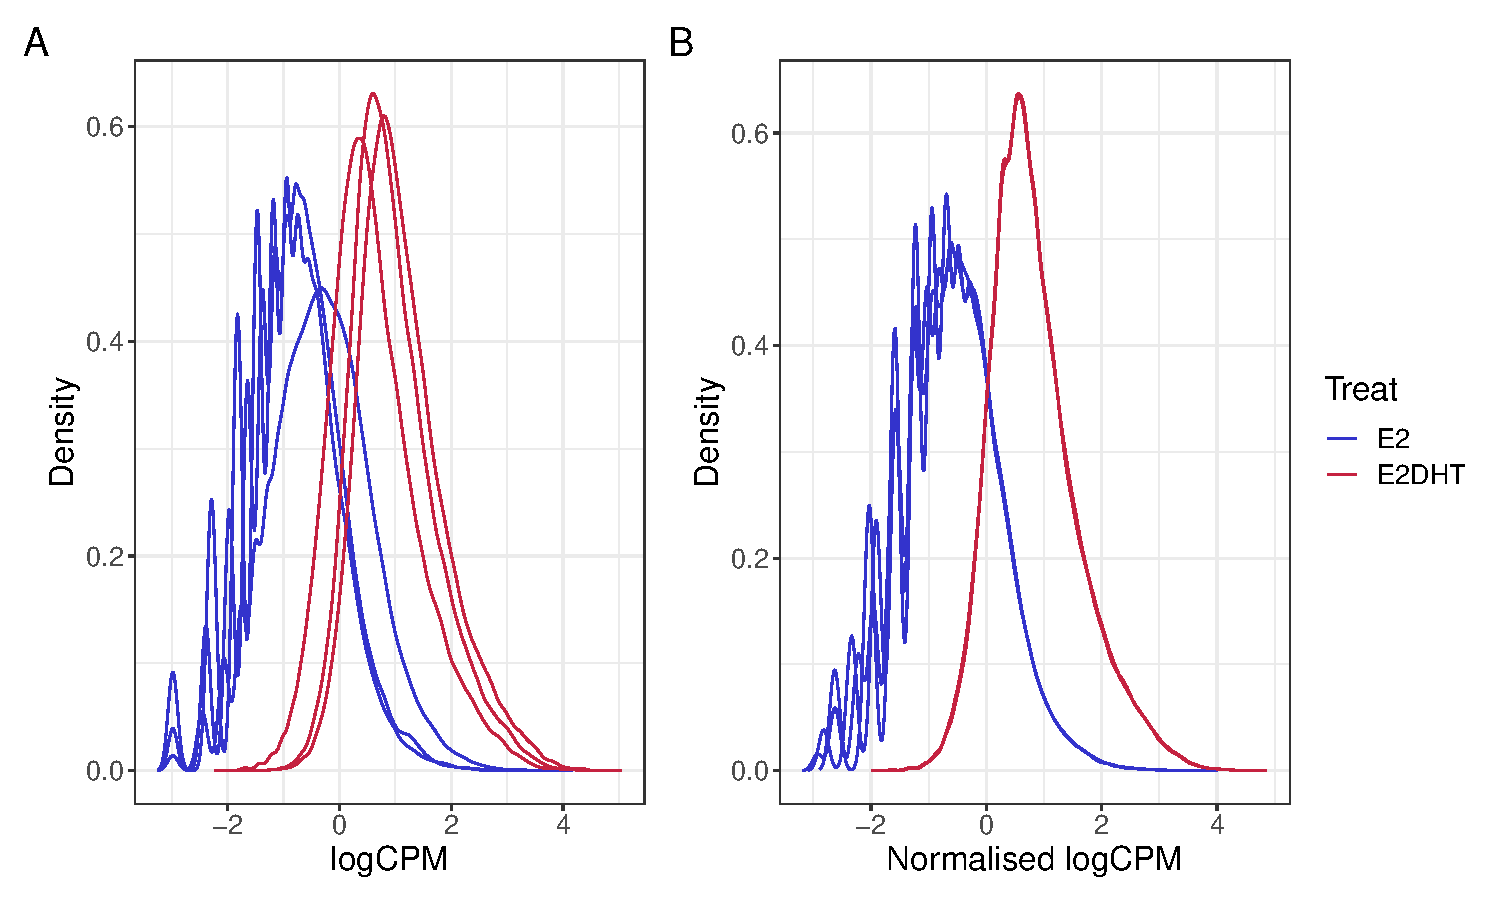
\includegraphics[width=\linewidth]{plot-logcpm-densities-1}
        \end{tikzfigure}		
        
           \begin{tikzfigure}[Partitioned $p$-values for H3K27ac Differential Signal Analysis based on co-detection of AR and ER. Here, 21\% more windows were considered significant\label{fig:ihw}]
	        	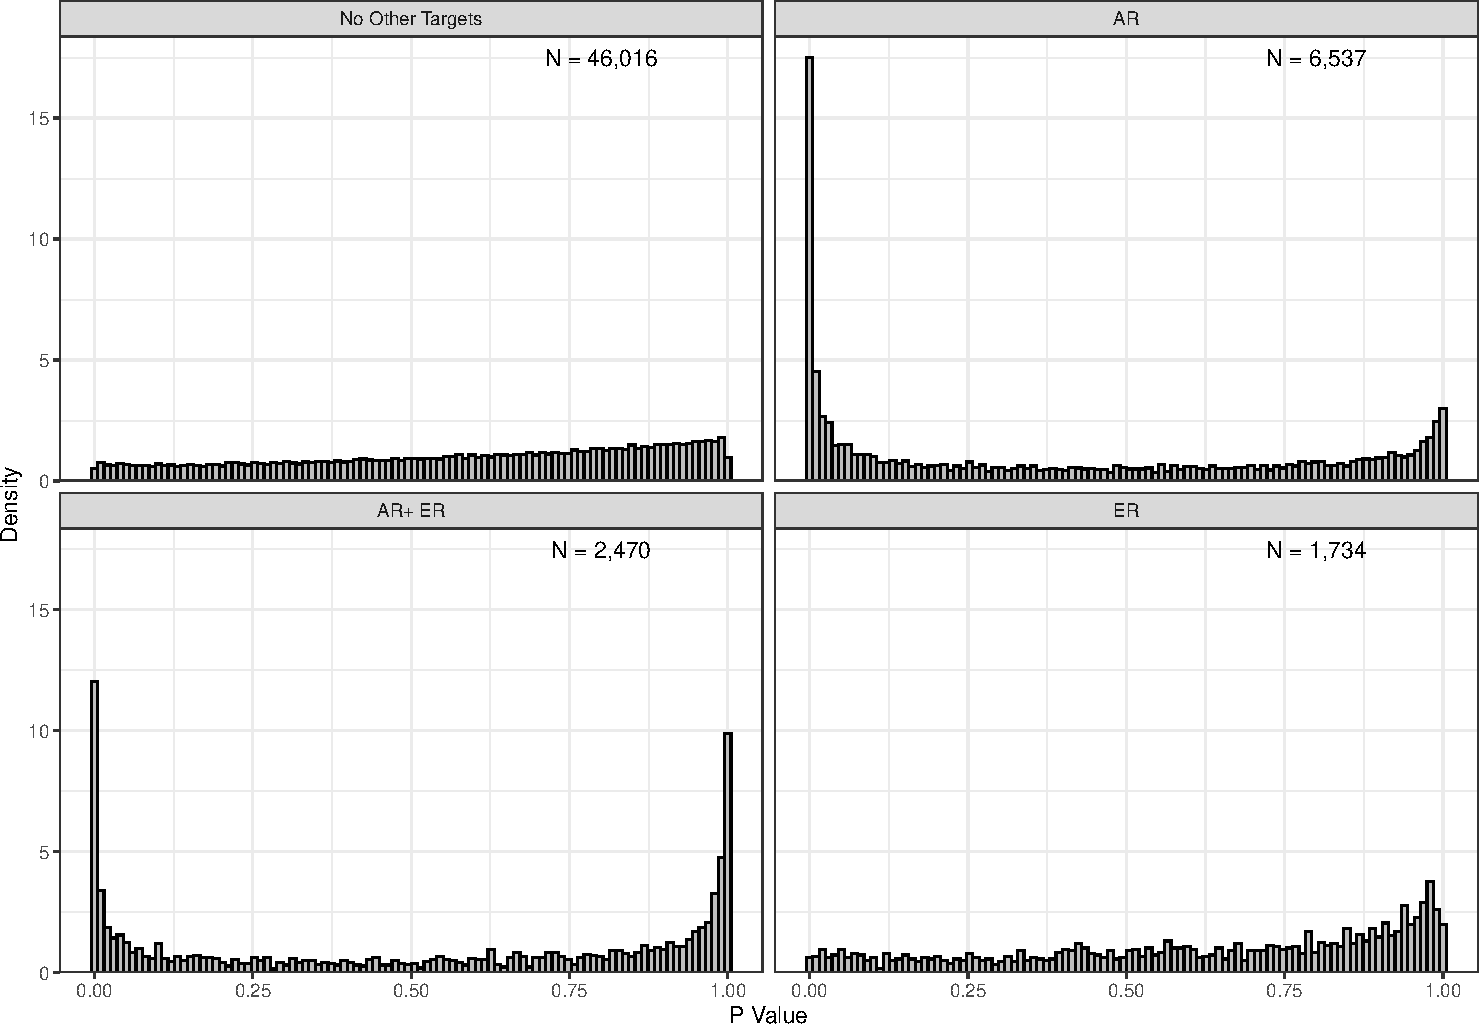
\includegraphics[width=\linewidth]{plot-ihw-pvals-1}
    	    \end{tikzfigure}	
        
	\end{minipage}    	

    	
    }

    \column{0.33}
    \block{Pairwise Comparisons}{
		\small
		\begin{minipage}{0.51\linewidth}
			\centering
			\begin{tikzfigure}[Pairwise DSA results for ER and H3K27ac]
	        	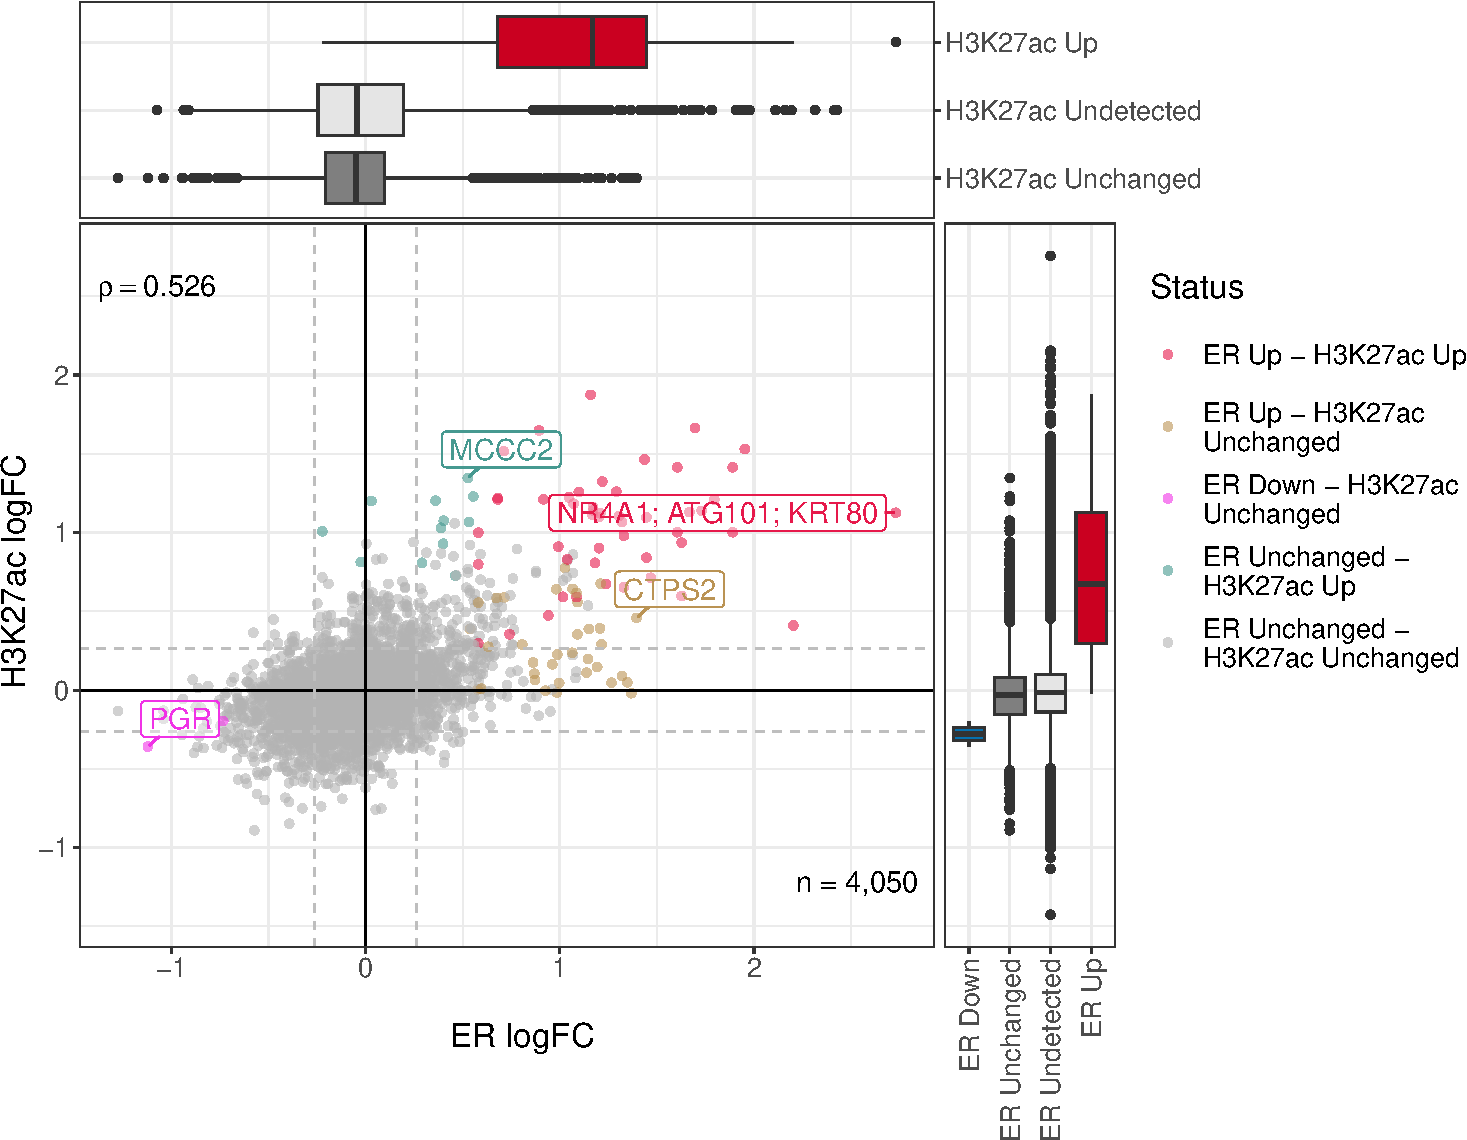
\includegraphics[width=0.9\linewidth]{plot-dbwin-1-crop}
    	    		\end{tikzfigure}			
	        
	        	\begin{tikzfigure}[DE Genes by combined AR and H3K27ac signal.\label{fig:volcano}]
			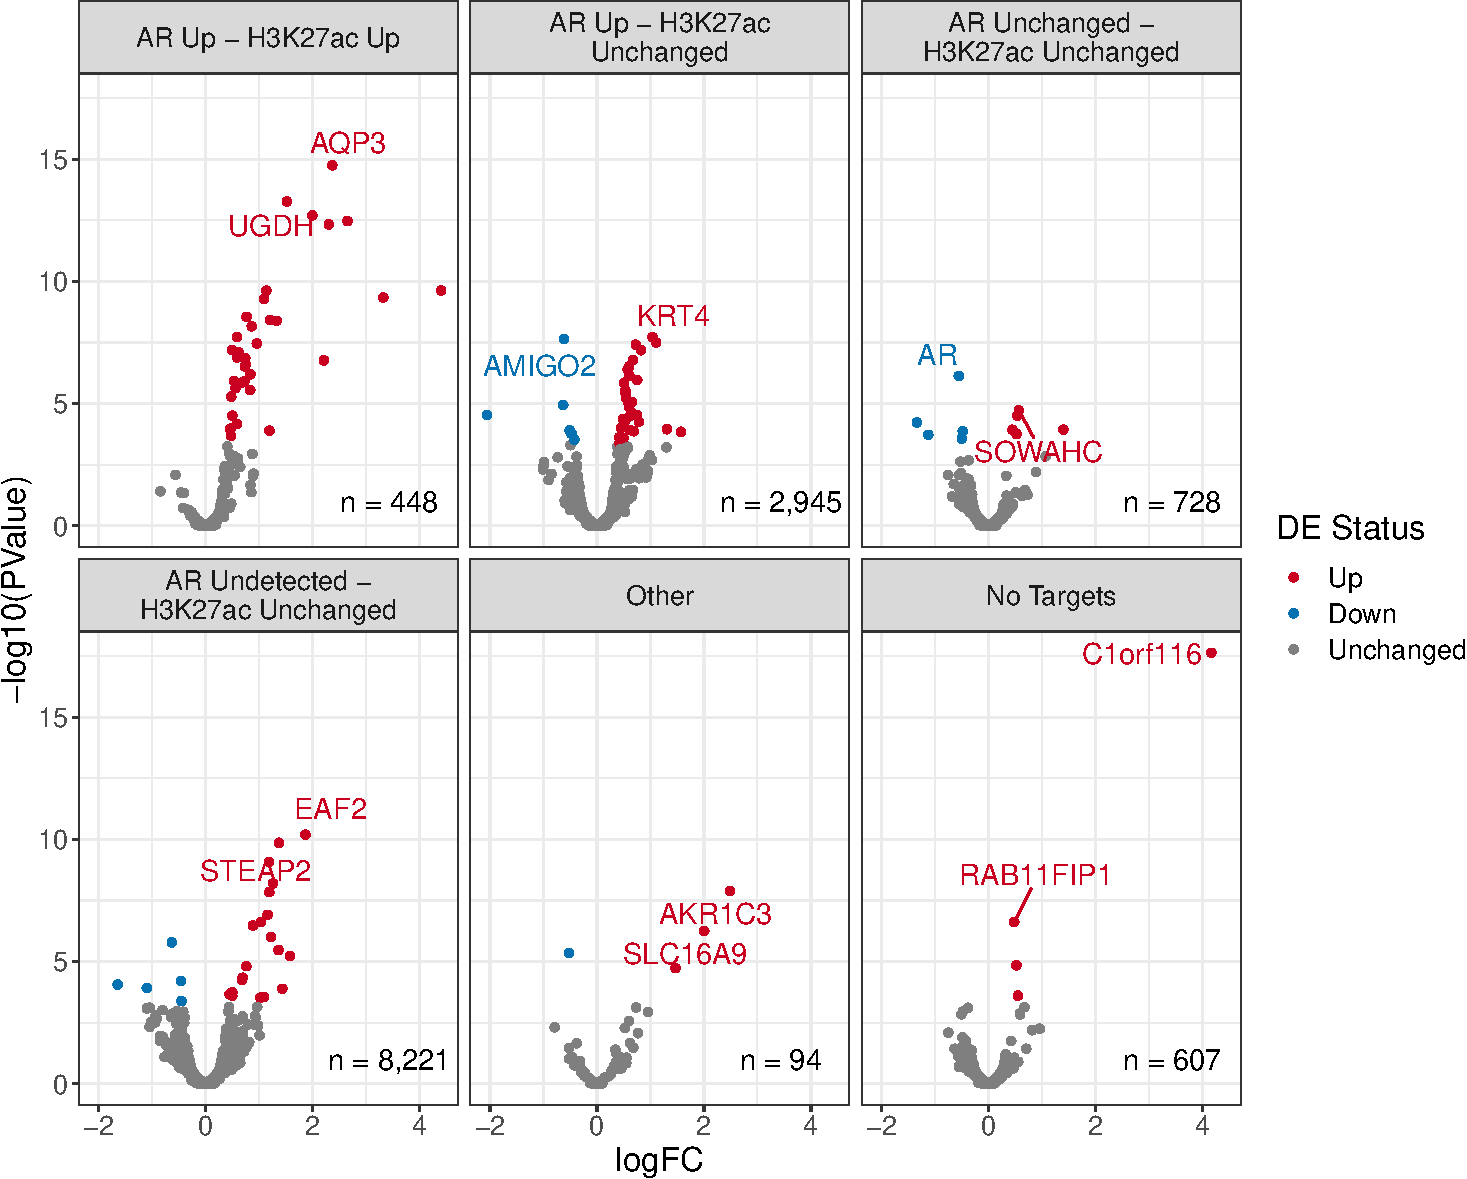
\includegraphics[width=0.9\linewidth]{plot-volcano-1-crop}
			\end{tikzfigure}	

    		\end{minipage}
		\begin{minipage}{0.49\linewidth}
			\centering
	    		\begin{tikzfigure}[Profile heatmap for sites showing increased signal for both AR and H3K27ac.]
	        	\includegraphics[width=\linewidth]{AR_Up_H3K27ac_Up_profile_heatmap-crop}
	        \end{tikzfigure}
    	    		
			\begin{tikzfigure}[Enrichment network for DGE results combined with sites showing a joint increase in AR and H3K27ac]
			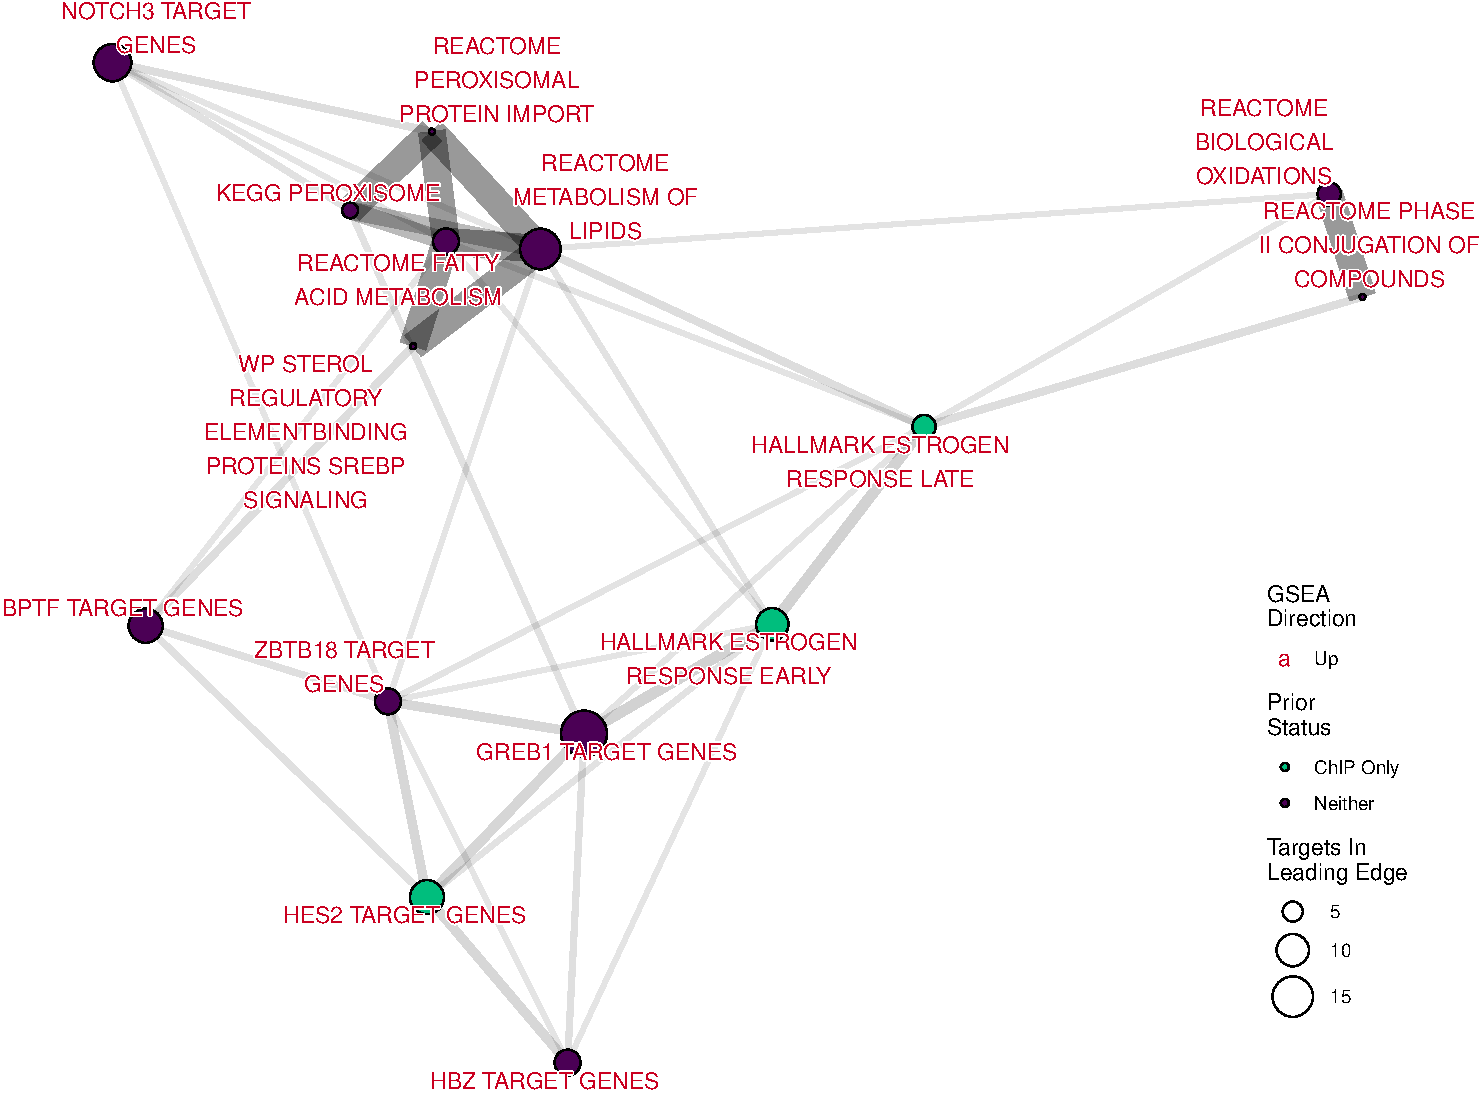
\includegraphics[width=\linewidth]{AR_Up-H3K27ac_Up_rnaseq_network-crop}
			\end{tikzfigure}					

    		\end{minipage}
    		\vspace{1cm}
    	\begin{minipage}{\linewidth}
    	\vspace{8mm}
    	\centering
    	\normalsize
    	All examples taken from an analysis of AR, ER and H3K27ac in ZR-75 cells treated with DHT
    	\end{minipage}

    \coloredbox{
	    \colorlet{innerblockbodybgcolor}{white}
		\begin{minipage}{0.79\linewidth}
	        \innerblock{\large \textbf{References}}{
		        \printbibliography[heading=none]
			}
		\end{minipage}
		\begin{minipage}{0.2\linewidth}
		    \innerblock[titlecenter]{\large See A Complete Report Here}{
		    \centering
		    
\includegraphics[width=0.85\linewidth]{gravi-example-qr-code.png} 
%		    \small
%		   	AR, ER \& H3K27ac\\[3mm]
%		    ZR-75-1 Cells\\[3mm]
%		    E2DHT vs E2\vspace{1cm}
	        }
		\end{minipage}
	 }
	    
    }


\end{columns}
\end{document}